\begin{figure*}[tp]
  \centering
  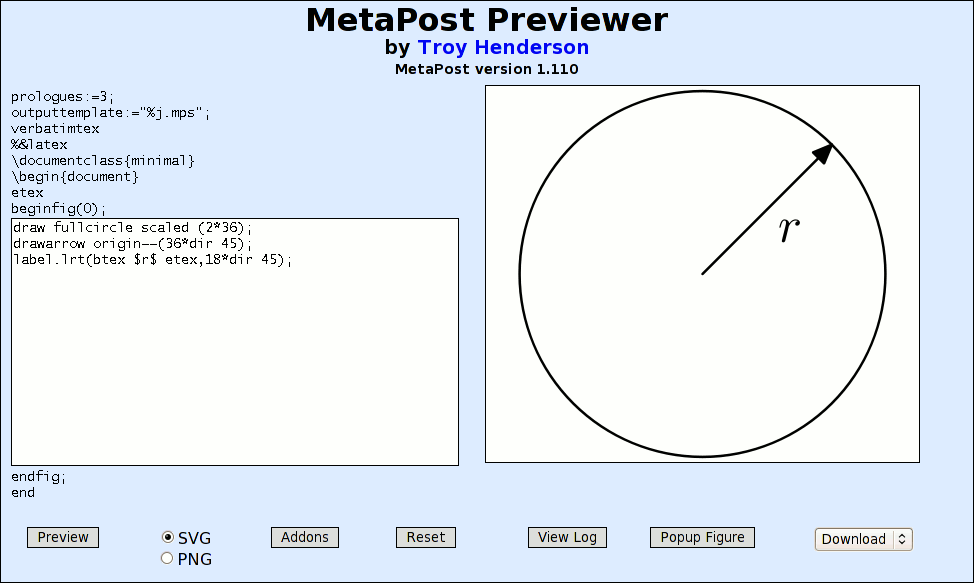
\includegraphics[width=\textwidth]{previewer}
  \caption{\MP{} Previewer}
  \label{fig:previewer}
\end{figure*}

\section{\MP{} compilation}
\label{sec:mpcompilation}

A typical \MP{} source file consists of one or more figures.
Compilation of the source file generates an \EPS{} graphic for each
figure.  These \EPS{} graphics are self-contained (i.e., the fonts used
in labels are embedded into the graphic) provided that |prologues:=3| is
declared.

If \File{foo.mp} is a typical \MP{} source file, then its contents are
likely of the following form:

\begin{lstlisting}[style=MP]
prologues:=3;
outputtemplate:="%j-%c.mps";
beginfig(1);
   |\normalfont\textit{draw commands}|
endfig;
beginfig(2);
   |\normalfont\textit{draw commands}|
endfig;
|\dots|
beginfig(|\normalfont$n$|);
   |\normalfont\textit{draw commands}|
endfig;
end
\end{lstlisting}

Executing

\begin{lstlisting}[style=text]
mpost foo.mp
\end{lstlisting}
yields the following output:

\begin{lstlisting}[style=text]
This is MetaPost, Version |\normalfont$\langle$\textit{version}$\rangle$|
(foo.mp [1] [2] |\normalfont\ldots| [|\normalfont$n$|] )
|\normalfont$n$| output files written: foo-1.mps .. foo-|\normalfont$n$|.mps
Transcript written on foo.log.
\end{lstlisting}

For users who just want to ``get started'' using \MP{}, a \MP{}
previewer is available at \url{http://www.tlhiv.org/mppreview}.  This
previewer (illustrated in \autoref{fig:previewer}) is simply a graphical
interface to \MP{} itself.  It generates a single graphic with the
option to save the output in \EPS{}, \PDF{}, and \SVG{} formats.  Users
may also choose to save the source code and can view the compilation log
to assist in debugging.
